\chapter{Sistema Desenvolvido}
\label{chap:sistema-desenvolvido}

Como exposto no Capítulo \ref{cap:dispositivos-protocolos}, são necessários vários protocolos ou adaptações para que a comunicação de um processo consiga atingir interoperabilidade entre o servidor e todos os dispositivos. Os sistemas \gls{SCADA} demonstrados no Capítulo \ref{cap:scada} utilizados para receber estas informações do servidor \gls{OPC} local ou diretamente destes dispositivos e organizá-las em um banco de dados, é a forma predominante na indústria e a forma mais confiável hoje. Todos os \textit{softwares} disponíveis para utilização que foram citados, tem em comum seu modo de funcionamento, onde é instalado em uma máquina próxima e fisicamente ligada ao processo, que por sua vez mantém todos os serviços necessários para o funcionamento integrado dos módulos que o compõe. Alguns dispõem de integração com o protocolo \gls{MQTT} e interfaceamento \gls{WEB}, mas não são nativamente desenvolvidos para o funcionamento remoto.

Este trabalho propõe o desenvolvimento de um sistema \gls{SCADA} \gls{WEB} em que sua distribuição não seja mais como os sistemas \gls{SCADA} citados, na forma de um Produto como Serviço onde o cliente paga por um \textit{software} desenvolvido e futuras atualizações que venham ocorrer mas fornece toda a estrutura necessária para o funcionamento dele, e sim \textit{Software} como Serviço, do inglês, \gls{SaaS}, em que a própria plataforma fornece os recursos necessários para a disponibilização de todos os módulos do sistema, sejam eles: servidores, segurança e atualizações do próprio \textit{software}.

Com a premissa de que toda a estrutura esteja disponível através da \textit{internet}, além de todas as funcionalidades de um sistema \gls{SCADA} convencional, várias vantagens podem ser listadas como:

\begin{alineascomponto}
    \item a capacitação profissional que antes seria necessária para a operação dessa estrutura é extremamente simplificada ao manuseio da interface;
    \item o gerenciamento é feito exclusivamente através do navegador podendo ser utilizado por todas as plataformas existentes na empresa, desde computadores, à \textit{smartphones} e \textit{tablets};
    \item com o uso da computação em nuvem, é possível a escalabilidade de recursos, sejam eles armazenamento ou processamento e tarefas simples que demandariam mais servidores ou a parada da aquisição de dados, podem agora ser feitas diretamente pela plataforma sem haver prejuízos ao processo;
    \item o mesmo sistema pode gerenciar múltiplos processos utilizando a mesma estrutura, podendo serem ou não apresentados na mesma interface;
    \item envio e recebimento de dados do processo podem ser feitos diretamente para a plataforma remota, desde que estejam disponíveis estas funcionalidades nos dispositivos citados no Capítulo \ref{cap:dispositivos-protocolos};
    \item com a possibilidade de uso de \textit{Web Service}, outros sistemas utilizados pela empresa podem trabalhar diretamente com o sistema \gls{SCADA}, obtendo informações ou atuando sobre o processo se necessário e desejado.
\end{alineascomponto}

Algumas desvantagens também são conhecidas inicialmente devido seu modo de funcionamento, como:

\begin{alineascomponto}
    \item existência de um tempo de atraso na casa de milisegundos entre o envio e o recebimento das informações entre e servidor e cliente devido a estrutura ser concebida de forma remota, relativamente longe do processo ao que seria a estrutura convencional;
    \item a dependência de uma boa conexão com a \textit{internet} e estabilidade desta para a utilização do sistema, que pode ser amenizada caso os dispositivos utilizados tenham uma memória local capaz de armazenar os dados no caso de uma queda na conexão por uma janela de tempo suficiente até o retorno desta;
    \item dispositivos que não tenham nativamente acesso à \textit{internet} deverão contar com drivers de comunicação capazes de intermediar estas informações ao sistema, como já acontece no \gls{SCADA} tradicional.

\end{alineascomponto}



\section{Aquisição de Dados}
\label{sec:aquisicao-dados}
O módulo mais importante para o funcionamento deste sistema é a aquisição de dados, pois através deles se dará o direcionamento de todos os outros módulos. Conforme descritos no Capítulo \ref{cap:dispositivos-protocolos}, os protocolos \gls{HTTP} e \gls{MQTT} são  projetados para \gls{WEB} e possuem compatibilidade com diversos formatos de dados, sendo este o motivo para escolha deles neste projeto. Será feita uma abstração da camada física de dispositivos que utilizem \gls{OPC} por exemplo, partindo do pressuposto que estes possuam drivers de comunicação que possam fazer envio destes dados pela \textit{internet}, ou seja, não haverá discriminação sobre os dados recebidos e tratados na plataforma. O utilizador da plataforma poderá escolher entre os dois protocolos de acordo com sua aplicação de interesse, abaixo são detalhados os processos referentes à aquisição de dados de cada um deles.

        \subsection{HTTP}
        \label{sec:aquisicao-http}
        O protocolo \gls{HTTP} será utilizado para a construção de uma \gls{API} baseada em \gls{REST} que possua a maior compatibilidade possível entre os métodos de chamada, para que até dispositivos simples possam trocar informações mesmo utilizando métodos de chamada triviais. Serão aceitos aqui, os três formatos de conteúdo descritos na seção \ref{sec:formatos-de-conteudo} devido o suporte nativo deste protocolo.
        
        Basicamente o processo de envio ou gerenciamento das informações contidas na plataforma, serão organizadas em 4 etapas: (i) Validação das Informações, (ii) Autenticação, (iii) Identificação das Informações, (iv) Banco de Dados, que serão detalhadas individualmente adiante. A Figura \ref{fig:figura-http-geral} traz um diagrama representando a sequência lógica destas quando iniciada a requisição.
        
        \begin{figure}[!h]
		\Caption{\label{fig:figura-http-geral} Diagrama das etapas do servidor para manipulação de dados.}
		%\centering
		\UFCfig{}{
			\fbox{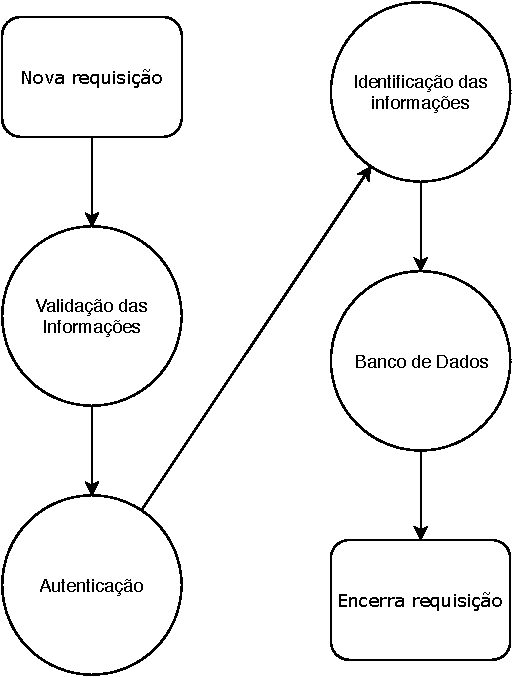
\includegraphics[width=8cm]{figuras/http-geral.pdf}}
		}{
			\Fonte{O autor}
		}	
    	\end{figure}
    	
    	\begin{figure}[!h]
		\Caption{\label{fig:figura-http-validacao} Diagrama de validação das informações recebidas.}
		%\centering
		\UFCfig{}{
			\fbox{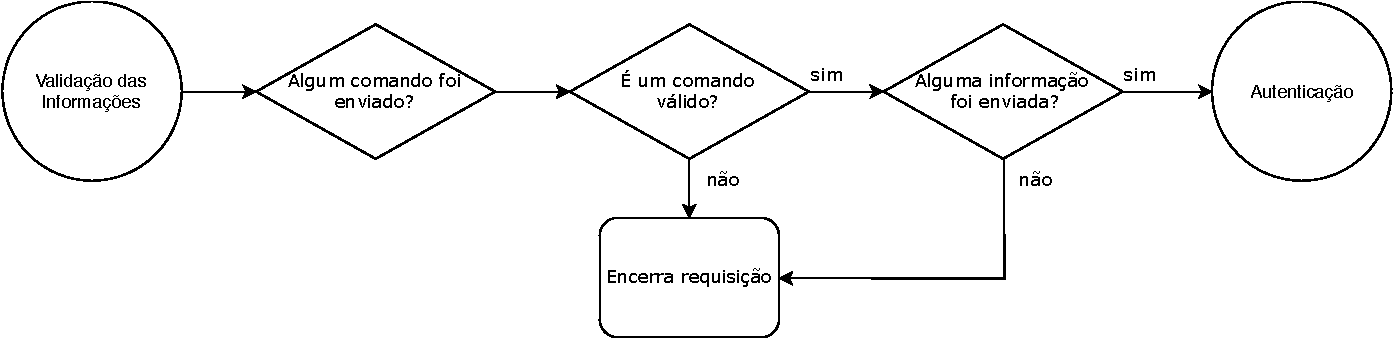
\includegraphics[width=15cm]{figuras/http-validacao.pdf}}
		}{
			\Fonte{O autor}
		}	
    	\end{figure}
    	
    	 Através de parâmetros configurados na \gls{URL} da \gls{API} da plataforma e cabeçalhos da requisição, o módulo identifica o método de chamada e qual comando o utilizador deseja. Se o comando enviado for reconhecido pelo módulo e exista alguma informação válida à ser enviada, é dado o direcionamento à etapa seguinte da Autenticação, caso contrário, a requisição é imediatamente encerrada. A Figura \ref{fig:figura-http-validacao} traz um diagrama com detalhes da etapa de validação das informações.
    	 
    	 Posteriormente, dentre os parâmetros enviados é feita uma verificação do \textit{token}, um código que funciona como uma senha e, caso seja válido e esteja autorizado ao uso da \gls{API}, o módulo verifica seu limite de envios no caso de novas inserções de informações e segue à próxima etapa caso esteja apto, encerrando a requisição caso contrário. A Figura \ref{fig:figura-http-autenticacao} traz um diagrama detalhando a lógica da autenticação.
    	
    	\begin{figure}[!h]
		\Caption{\label{fig:figura-http-autenticacao} Diagrama de autenticação do usuário.}
		%\centering
		\UFCfig{}{
			\fbox{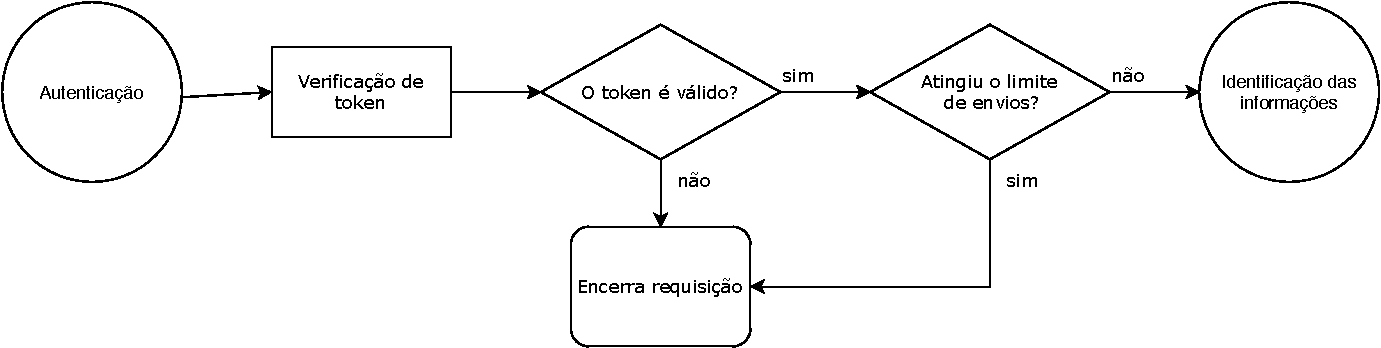
\includegraphics[width=15cm]{figuras/http-autenticacao.pdf}}
		}{
			\Fonte{O autor}
		}	
    	\end{figure}
    	
    	 Na etapa de Identificação do tipo de informação enviada, basicamente são listadas todas as variáveis que se deseja inserir ou modificar no banco de dados e a categorização delas, sejam: númericas, binárias ou texto. A Figura \ref{fig:figura-http-identificacao} traz detalhes sobre a identificação das informações provenientes da requisição.
    	
    	\begin{figure}[!h]
		\Caption{\label{fig:figura-http-identificacao} Diagrama sobre a identificação do tipo das informações.}
		%\centering
		\UFCfig{}{
			\fbox{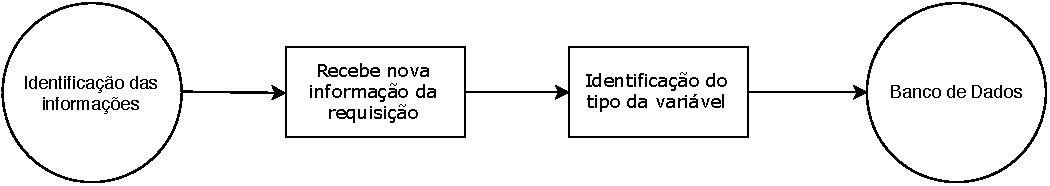
\includegraphics[width=15cm]{figuras/http-identificacao.pdf}}
		}{
			\Fonte{O autor}
		}	
    	\end{figure}
    	
    	Por último, são verificadas uma a uma se o nome das variáveis já estão cadastrados no banco de dados e dados o direcionamento para elas, repetindo a etapa de identificação para cada informação enviada, encerrando a requisição após o tratamento de todas elas. A Figura \ref{fig:figura-http-banco} traz mais detalhes sobre a etapa do banco de dados.
    	
    	\begin{figure}[!h]
		\Caption{\label{fig:figura-http-banco} Diagrama da etapa de banco de dados.}
		%\centering
		\UFCfig{}{
			\fbox{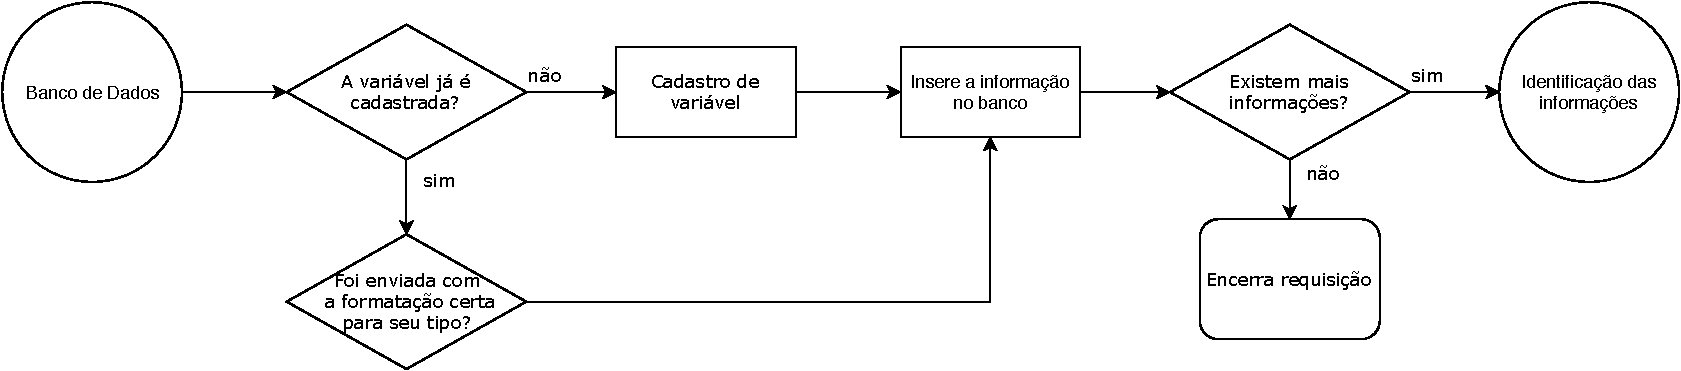
\includegraphics[width=15cm]{figuras/http-banco.pdf}}
		}{
			\Fonte{O autor}
		}	
    	\end{figure}
        
        \subsection{MQTT}
        \label{sec:aquisicao-mqtt}
        O protocolo \gls{MQTT} será utilizado para o envio e recebimento de informações de dispositivos que tenham restrição de largura de banda ou que tenham suporte nativo à sua utilização, devido sua facilidade de uso. Se faz necessária uma aplicação \textit{broker} para o funcionamento deste serviço e, devido ser um projeto de código aberto, foi escolhido o \textit{software} VerneMQ para esta finalidade. O projeto foi desenvolvido para ser distribuído, ou seja, há a possibilidade de escalabilidade vertical (quando se inclui mais servidores para a manutenção do serviço) e horizontal (quando se aumenta os recursos de um único servidor), em conformidade com o avanço da utilização crescente deste protocolo com a introdução da \textit{internet} das coisas. Além disto, traz funcionalidades como: autenticação, criptografia, níveis de serviço, envio de mensagens \textit{offline}, balanceamento de recursos, entre outros \cite{VerneMQ}.
        
        \begin{figure}[!h]
		\Caption{\label{fig:figura-mqtt-servico} Projeto utilizado para manter o serviço do MQTT.}
		%\centering
		\UFCfig{}{
			\fbox{
\includegraphics[width=10cm]{figuras/vernemq.png}}
		}{
			\Fonte{Adaptado de \cite{VerneMQ}}
		}	
    	\end{figure}
    	
    	Conforme explicado na seção \ref{sec:mqtt}, o MQTT recebe e envia informações através de tópicos e, no caso desta plataforma, para o envio de informações, são considerados: tópico como o \textit{token} do usuário e sub-tópico como a variável cadastrada no projeto em que se deseja inserir no banco de dados, simplificando portanto a autenticação deste serviço e tornando similar o uso da \gls{API} \gls{HTTP}. O módulo de aquisição de dados para o MQTT funciona como um subscritor neste serviço, capturando as informações enviadas pelo usuário e inserindo-as no banco de dados caso sejam válidas, o retorno de informação é dado pelo mesmo canal de envio. Os níveis de qualidade de serviço para a entrega das mensagens podem ser utilizados à critério de projeto pelo usuário.

    \section{Armazenamento dos Dados}
    \label{sec:armazenamento-dados}
    
    Os dados enviados para a plataforma, serão tratados e inseridos em um banco de dados relacional, contendo chave e valor, onde é dada para o usuário uma ideia de variável de programação para a chave. Também, são descritos tipos de variáveis em que sua utilização serão considerados, como exemplo de uma chave liga/desliga que poderá utilizar uma variável binária. Mais detalhes sober o funcionamento de cada tipo de variável e o banco de dados utilizado são dados abaixo.
    
        \subsection{Tipos de Variáveis}
        \label{sec:tipos-variaveis}
            
        \begin{alineascomponto}
            \item Binária: 
            \item Numérica: 
            \item Texto: 
        \end{alineascomponto}
        
        \subsection{Banco de Dados}
        \label{sec:banco-dados}
        oi
        
        \subsubsection{Tempo}
        \label{sec:tempo}
        oi
    
\section{Segurança}
    \label{sec:seguranca}
    oi
        
        \subsection{Proteções}
        \label{sec:protecoes}
        oi
        
        \subsection{Criptografia}
        \label{sec:criptografia}
        oi
        
        \subsection{Controle de Acesso}
        \label{sec:controle-acesso}
        oi
        
\section{Recursos Computacionais}
\label{sec:recursos-computacionais }
oi

    \subsection{Armazenamento}
    \label{sec:armazenamento}
    oi
    
    \subsection{Processamento}
    \label{sec:processamento}
    oi

\section{Plataforma Estudantil}
\label{sec:plataforma-estudantil}
oi